\chapter{Vector Spaces, Algebras, and Normed Spaces}
\pagenumbering{arabic}

\noindent For the entirety of this chapter assume $F$ to be  $\bfR$ or $\bfC$.

\section{Vector Spaces}
    \begin{definition}
        A \textit{vector space} (or \textit{linear space}) over $F$ is a nonempty set $V$ equipped with two operations:
            \begin{equation*}
            \begin{split}
                V \times V \xrightarrow{+} V &\mtext{defined by} (v,w) \mapsto v+w \\
                F \times V \rightarrow V &\mtext{defined by} (\alpha,v) \mapsto \alpha v
            \end{split}
            \end{equation*}
        satisfying:
            \begin{enumerate}[label = (\arabic*),itemsep=1pt,topsep=3pt]
                \item $(V, +)$ is an abelian group:
                    \begin{enumerate}[label = (\roman*),itemsep=1pt,topsep=3pt]
                        \item $u + (v+w) = (u+v) + w$ for all $u,v,w \in V$;
                        \item there exists $0_V$ such that $v + 0_V = 0_V + v = v$ for all $v \in V$;
                        \item for all $v \in V$, there exists $w \in V$ satisfying $v+w = w+v = 0_V$;
                        \item $v + w = w+v$ for all $v,w \in V$;
                    \end{enumerate}

                \item $(\alpha + \beta)v = \alpha v + \beta v$ for all $\alpha,\beta \in F$, $v \in V$;
                \item $\alpha(\beta v) = (\alpha \beta)v$ for all $\alpha,\beta \in F$, $v \in V$;
                \item $\alpha(v+w) = \alpha v + \alpha w$ for all $\alpha \in F$, $v,w \in V$;
                \item $1_F v = v$ for all $v \in V$.
            \end{enumerate}
    \end{definition}

    It can be shown that the vector $0_V$ is unique, the additive inverse in (iii) is unique (which we denote as $-v$), that $0v = 0_V$, and $(-1)v = -v$.

    \begin{exercise}
        Show (iv) follows from the other axioms.
    \end{exercise}

    \begin{exercise}
        Show $nv = \underbrace{v + v + ... + v}_{n \hspace{-4pt}\mtext{times}}$ for $n \in \bfZ_{\geq 1}$.
    \end{exercise}

    It can be shown that a subspace is a vector space in its own right.

    \begin{example}
        Let $\{W_i\}_{i \in I}$ be a family of vector spaces. Then $\bigcap_{i \in I}W_i$ is also a vector space.
    \end{example}

    \begin{example}
        Planes and lines through the origin are subspaces of $\bfR^3$.
    \end{example}

    \begin{definition}
        Let $V$ be a vector space and $S \subseteq V$ a subset.
            \begin{enumerate}[label = (\arabic*),itemsep=1pt,topsep=3pt]
                \item A \textit{linear combination} from $S$ is a finite sum $\sum_{j = 1}^n \alpha_j v_j$ with $\alpha_j \in F$, $v_j \in S$.
                \item The \textit{linear span} of $S$ is:
                    \begin{equation*}
                    \begin{split}
                        \Span(S) := \left\{ \sum_{j = 1}^n \alpha_j v_j \hspace{4pt}\middle|\hspace{4pt} n \in \bfN, \alpha_j \in F, v_j \in S \right\}.
                    \end{split}
                    \end{equation*}
            \end{enumerate}
    \end{definition}

    \begin{exercise}
        Show that $\Span(S) \subseteq V$ is a subspace and:
            \begin{equation*}
            \begin{split}
                \Span(S) = \bigcap \hspace{2pt}\{W \mid S \subseteq W, W \hspace{-2pt}\mtext{is a subspace}\hspace{-4pt}\},
            \end{split}
            \end{equation*}
        that is, $\Span(S)$ is the smallest subspace of $V$ containing $S$.
    \end{exercise}

    \begin{definition}
        Let $V$ be a vector space and $S \subseteq V$ a subset.
            \begin{enumerate}[label = (\arabic*),itemsep=1pt,topsep=3pt]
                \item $S$ is \textit{spanning} for $V$ if $\Span(S) = V$.
                \item $S$ is \textit{independent} if, given $n \in \bfN$, $\alpha_1,...,\alpha_n \in F$, $v_1,...,v_n \in S$, then $\sum_{j = 1}^n \alpha_j v_j = 0$ implies $\alpha_j = 0$ for all $j$.
            \end{enumerate}
    \end{definition}

    \begin{center}
        \begin{tikzpicture}
            \draw[thick] (0.3,0) -- (2.3,0);
            \node at (2.39, 0) {$/\,$};
            \node at (2.56, 0) {$/\,$};
            \draw[thick] (2.6,0) -- (4.6,0);
        \end{tikzpicture}
    \end{center}

    Our goal is to show that every vector space admits a basis. As such, recall the following definitions from a standard course in Real Analysis.

    \begin{definition}
        An \textit{ordering} on a set $X$ is a relation $R \subseteq X \times X$ on $X$ that is reflexive, transitive, and antisymmetric. We write $xRy$ as $x \leq_R y$. The pair $(X,\leq_R)$ is called an \textit{ordered set}. An ordering $\leq$ on $X$ is called \textit{total} (or \textit{linear}) if for all $x,y \in X$, $x \leq y$ or $y \leq x$.
    \end{definition}

    Note that if $(X,\leq)$ is an ordered set and $Y \subseteq X$ is a subset, then $(Y,\leq)$ is an ordered set as well.

    \begin{definition}
        Let $(X, \leq)$ be an ordered set and $Y \subseteq X$. An \textit{upper bound} for $Y$ is an element $u \in X$ with $u \geq y$ for all $y \in Y$. An element $m \in X$ is called \textit{maximal} if $x \in X$, $x \geq m$ implies $x = m$.
    \end{definition}

    \begin{lemma}[Zorn's Lemma]
        Let $(X,\leq_X)$ be an ordered set. Suppose every subset $Y \subseteq X$ for which $(Y,\leq_X)$ is totally ordered has an upper bound in $X$. Then $X$ admits a maximal element.
    \end{lemma}

    The proof of Zorn's Lemma is outside the interest of this text. 

    \begin{theorem}
        Every vector space admits a basis. Moreover, every independent set is contained in a basis.
    \end{theorem}
        \begin{proof}
            Let $S \subseteq V$ be linearly independent. Define:
                \begin{equation*}
                \begin{split}
                    \fT(S) = \{T \subseteq V \mid S \subseteq T, T \hspace{-3pt}\mtext{linearly independent}\hspace{-5pt}\}.
                \end{split}
                \end{equation*}
            Let $\fC \subseteq \fT(S)$ be a totally ordered subset. Set $R = \bigcup_{T \in \fC} T$. Clearly $R \supseteq S$. Assume $\sum_{j = 1}^n \alpha_j v_j = 0$, where $\alpha_j \in F$ and $v_j \in R$. Since $\fC$ is totally ordered, there exists $T_0 \in \fC$ with $v_j \in T_0$ for all $j = 1,...,n$. Since $T_0$ is independent, $\alpha_j = 0$ for all $j = 1,...,n$. Thus $R$ is independent as well. Whence $R$ is an upper bound for $\fC$. By Zorn's Lemma, $\fT(S)$ admits a maximal element, call it $B$.

            Claim: $B$ is a basis for $V$. Suppose towards contradiction it's not, then there exists $v_0 \in V \setminus \Span(B)$. Consider $B \cup \{v_0\}$ and let $\alpha_0 v_0 + \sum_{j = 1}^n \alpha_j v_j = 0_V$. If $\alpha_0 \neq 0$, then $\sum_{j = 1}^n \alpha_j v_j = -\alpha_0 v_0 $, giving $v_0 \in \Span(B)$ which is a contradiction. If $\alpha_0 = 0$, then $\sum_{j = 1}^n \alpha_j v_j = 0_V$. Since $B$ is independent, $\alpha_j = 0$ for all $j =1,...,n$. Thus $B \cup \{v_0\}$ is independent, contradicting the maximality of $B$. Whence $B$ is a basis for $V$.
        \end{proof}

    \begin{theorem}
        If $B_1$ and $B_2$ are bases for $V$, then $\card(B_1) = \card(B_2)$.
    \end{theorem}

    \begin{definition}
        If $V$ is a vector space, its \textit{dimension} is the cardinality of any of its bases.
    \end{definition}

    \begin{corollary}
        If $B$ is a basis for $V$, then every $v \in V$ can be written $v = \sum_{j = 1}^n \alpha_k \beta_k$, $\alpha_k \in F$, $b_k \in B$ in a unique way.
    \end{corollary}

    \begin{theorem}
        Let $V$ be a linear space and $B \subseteq V$ a subset. The following are equivalent:
            \begin{enumerate}[label = (\arabic*),itemsep=1pt,topsep=3pt]
                \item $B$ is a basis for $V$;
                \item $B$ is a maximal element in $\fT = \{T \subseteq V \mid \hspace{-4pt}\mtext{$T$ independent}\hspace{-4pt}\}$;
                \item $B$ is a minimal element in $\fS = \{S \subseteq V \mid \hspace{-4pt}\mtext{$S$ spans $V$}\hspace{-4pt}\}$;
            \end{enumerate}
    \end{theorem}

    \begin{definition}
        Let $\{V_i\}_{i \in I}$ be a family of vector spaces over a field $F$.
            \begin{enumerate}[label = (\arabic*),itemsep=1pt,topsep=3pt]
                \item The \textit{product} of $\{V_i\}_{i \in I}$ is denoted:
                    \begin{equation*}
                    \begin{split}
                        \prod_{i \in I}V_i := \{(v_i)_{i \in I} \mid v_i \in V_i\}.
                    \end{split}
                    \end{equation*}
                \item The \textit{co-product} (or \textit{sum}) is denoted 
                    \begin{equation*}
                    \begin{split}
                        \bigoplus_{i \in I}V_i := \left\{(v_i)_{i \in I} \mid v_i \in V_i,\hspace{2pt} \supp\bigl((v_i)_{i \in I}\bigr) <\infty \right\}.
                    \end{split}
                    \end{equation*}
            \end{enumerate}
    \end{definition}
    
    \begin{exercise}
        \phantom{a}
        \begin{enumerate}[label = (\arabic*),itemsep=1pt,topsep=3pt]
            \item Show that $\prod_{i \in I}V_i$ equipped with pointwise operations:
                \begin{equation*}
                \begin{split}
                    (v_i)_{i \in I} + (w_i)_{i \in I} &= (v_i + w_i)_{i \in I} \\
                    \alpha(v_i)_{i \in I} &= (\alpha v_i)_{i \in I}
                \end{split}
                \end{equation*}
            is a linear space.

            \item Show that $\bigoplus_{i \in I}V_i$ is a subspace of $\prod_{i \in I}V_i$.
        \end{enumerate}
    \end{exercise}

    \begin{proposition}
        Let $V$ be a vector space over $F$ and $W \subseteq V$. The (additive, abelian) quotient group $V/W$ can be made into a vector space by defining multiplication by scalars as $\alpha(v + W) = \alpha v + W$ for all $\alpha \in F$, $v + W \in V/W$.
    \end{proposition}

    \begin{example}
        \phantom{a}
        \begin{enumerate}[label = (\arabic*),itemsep=1pt,topsep=3pt]
            \item The set $F^n = \{(x_1,...,x_n) \mid x_j \in F\}$ with component-wise operations is a vector space.
            \item The set $M_{n,m}(F) = \{(a_{ij}) \mid a_{ij} \in F\}$ with linear operations is a vector space.
            \item Let $\Omega$ be a nonempty set. Then $\cF(\Omega,F) = \{f \mid f:\Omega \rightarrow F\}$ with pointwise operations is a vector space.
            \item The set $\ell_\infty(\Omega,F) = \{f \in \cF(\Omega,F) \mid \lnorm f \rnorm _u < \infty \}$ with pointwise operations is a vector space.
                \begin{exercise}
                    Show $\ell_\infty(\Omega,F) \subseteq \cF(\Omega,F)$ is a subspace.
                \end{exercise}

            \item Let $f:[a,b] \rightarrow \bfR$ be any function. Let $\cP = \{a = x_0 < x_1 < ... < x_{n-1} < x_n = b\}$ be a partition of $[a,b]$. The \textit{variation of $f$ on $\cP$} is defined as:
            \begin{equation*}
            \begin{split}
                \text{Var}(f;\cP) = \sum_{k = 1}^n |f(x_k) - f(x_{k-1})|.
            \end{split}
            \end{equation*}
        We say $f$ is a \textit{bounded variation} if:
            \begin{equation*}
            \begin{split}
                \text{Var}(f) := \sup_{\cP}\text{Var}(f;\cP) < \infty.
            \end{split}
            \end{equation*}
        The set of all functions of bounded variation is defined:
            \begin{equation*}
            \begin{split}
                \text{BV}([a,b]) = \{f:[a,b] \rightarrow \bfR \mid \text{Var}(f) < \infty\}.
            \end{split}
            \end{equation*}
        This is a vector space by defining addition and scalar multiplication componentwise.
            \begin{exercise}\label{ex:bv-subspace}
                Show that $\text{BV([a,b])} \subseteq \ell_\infty([a,b],\bfR)$ is a subspace.
            \end{exercise}

            \item Let $K \subseteq V$ be a convex subset of a vector space $V$, that is, for all $v,w \in K$ and $t \in [0,1]$, then $(1-t)v + tw \in K$. A function $f:K \rightarrow F$ is said to be \textit{affine} if $x,y \in K$ and $t \in [0,1]$ implies $f((1-t)x + ty) = (1-t)f(x) + tf(y)$. The set \newline $\text{Aff}(K,F) = \{f \in \cF(\Omega,F) \mid f \hspace{3pt}\text{affine}\hspace{1pt}\}$ with pointwise operations is a vector space.
                \begin{exercise}
                    Show $\text{Aff}(\Omega,F) \subseteq \cF(\Omega,F)$ is a subspace.
                \end{exercise}
            \item The set $C([a,b],F) = \{f:[a,b] \rightarrow F \mid f \hspace{3pt}\text{continuous}\hspace{1pt}\}$ with pointwise operations is a vector space.
                \begin{exercise}
                    Explain why $C([a,b],F) \subseteq \ell_\infty([a,b],F)$ is a subspace.
                \end{exercise}
            \item Consider the following sequence spaces:
                \begin{itemize}
                    \item $s = \{(a_k)_k \mid a_k \in F\} = \cF(\bfN,F)$;
                    \item $\ell_\infty = \ell_\infty(\bfN,F) = \{(a_k)_k \mid \sup_{k \geq 1}|a_k| < \infty\}$;
                    \item $c = \{(a_k)_k \mid (a_k)_k \hspace{3pt}\text{converges}\hspace{2pt}\}$;
                    \item $c_0 = \{(a_k)_k \mid (a_k)_k \rightarrow 0\}$;
                    \item $c_{00} = \{(a_k)_k \mid \supp\bigl((a_k)_k\bigr) < \infty\}$;
                    \item $\ell_1 = \left\{ (a_k)_k \mid \sum_{k = 1}^\infty |a_k| < \infty \right\}$.
                \end{itemize}
            These are all vector spaces with pointwise operations. In fact, $c_{00} \subseteq c_0 \subseteq c \subseteq \ell_\infty \subseteq s$ are all subspaces.
                \begin{exercise}
                    Show that $\ell_1 \subseteq c_0$ is a subspace.
                \end{exercise}

            \item Consider the following continuous function spaces on $\bfR$:
                \begin{itemize}
                    \item $C(\bfR) = \{f:\bfR \rightarrow F \mid f \hspace{3pt}\text{continuous}\hspace{2pt}\}$;
                    \item $C_b(\bfR) = C(\bfR) \cap \ell_\infty(\bfR)$;
                    \item $C_0(\bfR) = \{f \in C(\bfR) \mid \limit_{x \rightarrow \pm\infty} f(x) = 0\}$;
                    \item Recall that a function is \textit{compactly supported} if for all $\epsilon > 0$, there exists $\alpha > 0$ such that $|x| \geq \alpha$ implies $f(x) = 0$. The set of compactly supported functions is denoted $C_c(\bfR) = \{f \in C(\bfR) \mid f \hspace{3pt}\text{compactly supported}\hspace{2pt}\}$.
                \end{itemize}
            These are all vector spaces with pointwise operations, and $C_c(\bfR) \subseteq C_0(\bfR) \subseteq C_b(\bfR) \subseteq C(\bfR)$ are all subspace inclusion.
        \end{enumerate}
    \end{example}

    \begin{definition}
        If $V$ and $W$ are linear spaces over a common field $F$, a map $T:V \rightarrow W$ is called \textit{linear} if $T(v_1 + \alpha v_2) = T(v_1) + \alpha T(v_2)$ for all $v_1,v_2 \in V$ and $\alpha \in F$.
    \end{definition}
    
    \begin{example}
        Let $A \in M_{m,n}(F)$. Then $T_A:F^n \rightarrow F^m$ defined by $T_A(v) = Av$ is linear. Let $\{e_1,...,e_n\}$ be a basis for $F^n$. If $T:F^n \rightarrow F^m$ is linear, set:
            \begin{equation*}
            \begin{split}
                [T] = \Bigl( T(e_1) \Bigm\vert T(e_2) \Bigm\vert \hspace{4.5pt}...\hspace{4.5pt}\Bigm\vert T(e_n) \Bigr).
            \end{split}
            \end{equation*}
        This gives $T(v) = [T]v$ for all $v \in F^n$. In fact, we also have $[T_A] = A$ and $T_{[T]} = T$.
    \end{example}

    \begin{example}
        The \textit{canonical projection} is linear:
            \begin{equation*}
            \begin{split}
                \pi_j: \prod_{i \in I}V_i \rightarrow V_j \mtext{defined by} \pi_j\bigl((v_i)_i\bigr) = v_i.
            \end{split}
            \end{equation*}
        We also have that the \textit{coordinate exclusions} are linear:
            \begin{equation*}
            \begin{split}
                \iota_j: V_j \hookrightarrow \bigoplus_{i \in I}V_i \mtext{defined by} \iota_j(v) = (v_i)_i \hspace{1.5pt}, \hspace{-2pt}\mtext{where} v_i = \begin{cases}
                    0_v, &i \neq j \\
                    v_j, &\text{otherwise}.
                \end{cases}
            \end{split}
            \end{equation*}
        The \textit{evaluation map} is linear as well. For $s \in S$, consider:
            \begin{equation*}
            \begin{split}
                e_s : \cF(S,F) \rightarrow F \mtext{defined by} e_s(f) = f(s).
            \end{split}
            \end{equation*}
    \end{example}

    \begin{proposition}
        Let $V$ be a vector space with basis $B$. Let $W$ be a vector space and suppose $\varphi:B \rightarrow W$ is a map. Then there exists a unique linear map $T_\varphi: V \rightarrow W$ with $T_\varphi(b) = \varphi(b)$ for all $b \in B$. We have the following diagram.
            \begin{center}
            \begin{tikzcd}
            B \arrow[rd, "\varphi"'] \arrow[r, "\iota", hook] & V \arrow[d, "T_\varphi", dotted] \\
                                                              & W                               
            \end{tikzcd}
            \end{center}
    \end{proposition}
        \begin{proof}
            Define $T_\varphi:V \rightarrow W$ by:
                \begin{equation*}
                \begin{split}
                    T_\varphi(v)
                    & = T_\varphi \left( \sum_{j = 1}^n \alpha_j b_j \right) \\
                    & = \sum_{j = 1}^n \alpha_j \varphi(b_j).
                \end{split}
                \end{equation*}
            Let $v_1,v_2 \in V$ and $c \in F$. We have that:
                \begin{equation*}
                \begin{split}
                    T_\varphi(v_1 + cv_2)
                    & = T_\varphi \left( \sum_{j = 1}^n \alpha_j b_j + c \sum_{j = 1}^n \beta_j b_j \right) \\
                    & = T_\varphi \left( \sum_{j = 1}^n (\alpha_j + c \beta_j)b_j \right) \\
                    & = \sum_{j  =1}^n (\alpha_j + c \beta_j)\varphi(b_j) \\
                    & = \sum_{j = 1}^n \alpha_j \varphi(b_j) + c \sum_{j =1}^n \beta_j \varphi(b_j) \\
                    & = T_\varphi(v_1) + c T_\varphi(v_2).
                \end{split}
                \end{equation*}
            Thus $T_\varphi$ is linear. Chasing the above diagram makes it clear that $T_\varphi(b) = \varphi(b)$. It remains to show that $T_\varphi$ is unique. Let $T$ be another linear transformation satisfying $T(b) = \varphi(b)$ for all $b \in B$. Then:
                \begin{equation*}
                \begin{split}
                    T(v)
                    & = T \left( \sum_{j = 1}^n \alpha_j b_j \right) \\
                    & = \sum_{j = 1}^n \alpha_j \varphi(b_j) \\
                    & = T_\varphi \left( \sum_{j = 1}^n \alpha_j b_j \right) \\
                    & = T_\varphi(v).
                \end{split}
                \end{equation*}
            Thus $T_\varphi$ is unique.
        \end{proof}

    \begin{proposition}
        Let $T:V \rightarrow W$ be linear.
            \begin{enumerate}[label = (\arabic*),itemsep=1pt,topsep=3pt]
                \item $\ker(T) = \{v \in V \mid T(v) = 0_W\}$ is a linear subspace of $V$.
                \item $\Image(T) = \{T(v) \mid v \in V\}$ is a linear subspace of $W$.
                \item $\ker(T) = \{0_V\}$ if and only if $T$ is injective.
                \item $\Image(T) = W$ if and only if $T$ is surjective.
            \end{enumerate}
    \end{proposition}
        \begin{proof}
            (1) Let $v_1,v_2 \in \ker(T)$ and $\alpha \in F$. Observe that:
                \begin{equation*}
                \begin{split}
                    T(v_1 + cv_2)
                    & = T(v_1) + cT(v_2) \\
                    & = 0.
                \end{split}
                \end{equation*}
            Thus $v_1 + cv_2 \in \ker(T)$, giving $\ker(T)$ as a linear subspace of $V$.

            (2) Let $w_1,w_2 \in \Image(T)$. Then there exists $v_1.v_2 \in V$ with $T(v_1) = w_1$ and $T(v_2) = w_2$. We have:
                \begin{equation*}
                \begin{split}
                    w_1 + cw_2 
                    & = T(v_1) + cT(v_2) \\
                    & = T(v_1 + cv_2).
                \end{split}
                \end{equation*}
            Whence $w_1 + cw_2 \in \Image(T)$, giving $\Image(T)$ as a linear subspace of $W$.

            (3) Let $\ker(T) = \{0\}$. Suppose $T(v_1) = T(v_2)$. Then $T(v_1) - T(v_2) = T(v_1 - v_2) = 0_W$. It must be that $v_1 -v_2 = 0_W$, giving $v_1 = v_2$. Thus $T$ is injective. Conversely, suppose $T$ is injective and let $v \in \ker(T)$. Then $T(v) = 0_W = T(0_V)$. Hence $v = 0_V$, establishing $\ker(T) = \{0\}$.

            (4) This is by definition of surjectivity.
        \end{proof}

    \begin{proposition}
        If $T:V \rightarrow W$ is linear and bijective, then the inverse map $T^{-1}:W \rightarrow V$ is linear.
    \end{proposition}
        \begin{proof}
            We have that:
                \begin{equation*}
                \begin{split}
                    T(T^{-1}(w_1) + \alpha T^{-1}(w_2)) = w_1 + \alpha w_2 = T \circ T^{-1}(w_1 + \alpha w_2).
                \end{split}
                \end{equation*}
            Applying $T^{-1}$ to both sides gives the desired result.
        \end{proof}

    \begin{proposition}[Vector Spaces are Injective]
        Let $U,V,W$ be vector spaces and $0 \rightarrow U \xrightarrow{j} V$ be exact (that is, $j$ is injective). Let $\varphi:U \rightarrow W$ be linear. There exists a linear map $\Psi:V \rightarrow W$ such that $\varphi = \Psi\circ j $; i.e., the following diagram commutes:
            \begin{center}
                \begin{tikzcd}
                    0 \arrow[r] & U \arrow[r, "j"] \arrow[d, "\varphi"'] & V \arrow[ld, "\Psi", dotted] \\
                                & W                                      &                             
                    \end{tikzcd}
            \end{center}
    \end{proposition}
        \begin{proof}
            Let $\{u_i\}_{i \in I}$ be a basis for $U$. We must first show that $\{j(u_i)\}_{i \in I}$ is linearly independent. Notice that:
                \begin{equation*}
                \begin{split}
                    0_V 
                    & = \sum_{i \in I}\alpha_i j(u_i) \\
                    & = j \left( \sum_{i \in I} \alpha_i u_i \right).
                \end{split}
                \end{equation*}
            By the injectivity of $j$, we have that $\sum_{i \in I}\alpha_i u_i = 0_U$. Thus $\alpha_i = 0$ for all $i \in I$, giving $\{j(u_i)\}_{i \in I}$ as linearly independent.

            Since $\{j(u_i)\}_{i \in I}$ is linearly independent in $V$, we can extend it to a basis \newline $B = \{v_i\}_{i \in J}$ where $I \subseteq J$ and $v_i = j(u_i)$ whenever $i \in I$. Now define $\psi:B\rightarrow W$ by:
                \begin{equation*}
                \begin{split}
                    \psi(v_i) = \begin{cases} \varphi(u_i), & i \in I \\ w, & i \in J\setminus I \h3, \end{cases}
                \end{split}
                \end{equation*}
            where $w \in W$ is arbitrary. Since this is a map of basis elements, there exists a unique linear map $\Psi:V \rightarrow W$ with $\Psi(v_i) = \psi(v_i)$ for all $v_i \in B$. We can finally see that:
                \begin{equation*}
                \begin{split}
                    \varphi(u_i)
                    & = \psi(v_i) \\
                    & = \Psi(v_i) \\
                    & = \Psi(j(u_i)).
                \end{split}
                \end{equation*}
            This establishes that $\varphi = \Psi \circ j$.
        \end{proof}

    \begin{proposition}[Vector Spaces are Projective]
        Let $U,V,W$ be vector spaces and $V \xrightarrow{\pi}U \rightarrow 0$ be exact (that is, $\pi$ is onto). Let $\varphi:W \rightarrow U$ be linear. There exists a linear map $\Psi:V \rightarrow W$ such that $\varphi = \pi \circ \Psi$; i.e., the following diagram commutes:
            \begin{center}
                \begin{tikzcd}
                    & W \arrow[d, "\varphi"] \arrow[ld, "\Psi"', dotted] &   \\
                    V \arrow[r, "\pi"] & U \arrow[r]                                        & 0
                \end{tikzcd}
            \end{center}
    \end{proposition}
        \begin{proof}
            Let $B = \{w_i\}_{i \in I}$ be a basis for $W$. Define $\psi:B \rightarrow V$ by $\psi(w_i) = \pi^{-1}(\varphi(w_i))$. Since this is a map of basis elements, it extends to a unique (dependent on $\pi^{-1}$) linear map $\Psi:W \rightarrow V$ with $\Psi(w_i) = \psi(w_i)$ for all $w_i \in B$. Moreover, we have that:
                \begin{equation*}
                \begin{split}
                    (\pi \circ \Psi)(w_i)
                    & = (\pi \circ \psi)(w_i) \\
                    & = (\pi \circ (\pi^{-1} \circ \varphi))(w_i) \\
                    & = \varphi(w_i). \qedhere
                \end{split}
                \end{equation*}
        \end{proof}

    \begin{definition}
        Let $V$ and $W$ be vector spaces over $F$. A \textit{linear isomorphism} between $V$ and $W$ is a bijective linear map $T:V \rightarrow W$. If such a $T$ exists, we say $V$ and $W$ are \textit{linearly isomorphic}, and write $V \cong W$.
    \end{definition}

    \begin{center}
        \begin{tikzpicture}
            \draw[thick] (0.3,0) -- (2.3,0);
            \node at (2.39, 0) {$/\,$};
            \node at (2.56, 0) {$/\,$};
            \draw[thick] (2.6,0) -- (4.6,0);
        \end{tikzpicture}
    \end{center}

    Finite dimensional vector spaces are boring. This is illustrated through the following theorem.

    \begin{theorem}
        Let $V$ and $W$ be finite-dimensional vector spaces over $F$. Then $V \cong W$ if and only if $\dim(V) = \dim(W)$.
    \end{theorem}
        \begin{proof}
            Suppose $V \cong W$. Then there is an isomorphism taking basis of $V$ to a basis of $W$. Therefore they have the same dimension.

            Conversely, if $\dim(V) = \dim(W) = n$, then they are each isomorphic to $F^n$, giving that they are isomorphic to eachother.
        \end{proof}

        \begin{center}
            \begin{tikzpicture}
                \draw[thick] (0.3,0) -- (2.3,0);
                \node at (2.39, 0) {$/\,$};
                \node at (2.56, 0) {$/\,$};
                \draw[thick] (2.6,0) -- (4.6,0);
            \end{tikzpicture}
        \end{center}

    \begin{example}
        Let $V$ be a vector space, $W \subseteq V$ a subspace. The \textit{natural projection}:
            \begin{equation*}
            \begin{split}
                \pi:V \rightarrow V/W \mtext{defined by}\pi(v) = v+W
            \end{split}
            \end{equation*}
        is a linear surjective map.
    \end{example}

    \begin{theorem}[First Isomorphism Theorem for Vector Spaces]
        Let $T:V \rightarrow V'$ be a linear map and $W \subseteq V$ a subspace.
        \begin{enumerate}[label = (\arabic*),itemsep=1pt,topsep=3pt]
            \item If $T$ "kills" $W$ (that is, $W \subseteq \ker(T)$), then there exists a linear map $\widetilde{T}:V/W \rightarrow V'$ with $\widetilde{T} \circ \pi = T$; i.e., the following diagram commutes.
                \begin{center}
                    \begin{tikzcd}
                        V \arrow[rr, "T"] \arrow[rd, "\pi"'] &                                & V' \\
                        & V/W \arrow[ru, "\widetilde{T}"', dotted] &   
                    \end{tikzcd}
                \end{center}

            \item If $\ker(T) = W$, then $\widetilde{T}$ is injective.
            \item If $\ker(T) = W$ and $\Image(T) = V'$, then $V/W \cong V'$.
        \end{enumerate}
    \end{theorem}
        \begin{proof}
            (1) As stipulated, define $\widetilde{T}(v+W) = T(v)$. We must show that $\widetilde{T}$ is well-defined: suppose $v_1 + W = v_2 + W$ for some $v_1,v_2 \in V$. Then $v_1 = v_2 + w$ for some $w \in W$. This gives:
                \begin{equation*}
                \begin{split}
                    \widetilde{T}(v_1 + W)
                    & = \widetilde{T}(v_2 + w + W) \\
                    & = \widetilde{T}(v_2 + W).
                \end{split}
                \end{equation*}
            Whence $\widetilde{T}$ is well-defined. Now given $v_1 + W, v_2 +W \in V/W$ and $\alpha \in F$, observe that:
                \begin{equation*}
                \begin{split}
                    \widetilde{T}\bigl((v_1 + W) + c (v_2 + W)\bigr)
                    & = \widetilde{T}\bigl( (v_1 + cv_2) + W\bigr) \\
                    & = T(v_1 + cv_2) \\
                    & = T(v_1) + cT(v_2) \\
                    & = \widetilde{T}(v_1 + W) + c \widetilde{T}(v_2 + W). 
                \end{split}
                \end{equation*}
            Thus $\widetilde{T}$ is linear.

            (2) If $\ker(T) = W$, then:
                \begin{equation*}
                \begin{split}
                    \ker(\widetilde{T})
                    & = \{v + W \mid \widetilde{T}(v+W) = 0_{V'}\} \\
                    & = \{v + W \mid T(v) = 0_{V'}\} \\
                    & = \{v + W \mid v \in \ker(T)\} \\
                    & = \{v + W \mid v \in W\} \\
                    & = \{0\}.
                \end{split}
                \end{equation*}
            Thus $\widetilde{T}$ is injective.

            (3) It remains to show that $\Image(T) = V'$ implies $\widetilde{T}$ is surjective. Observe that:
                \begin{equation*}
                \begin{split}
                    \Image(\widetilde{T})
                    & = \{\widetilde{T}(v+W) \mid v+W \in V/W \} \\
                    & = \{\widetilde{T}(\pi(v)) \mid v \in V \} \\
                    & = \{T(v) \mid v \in V\} \\
                    & = \Image(T) \\
                    & = V'.
                \end{split}
                \end{equation*}
            Thus $\widetilde{T}$ is surjective, which establishes it as a bijection. This gives $V/W \cong V'$.
        \end{proof}

    \begin{definition}
        Let $S$ be a nonempty set. The \textit{free vector space} of $S$ is:
            \begin{equation*}
            \begin{split}
                \bfF(S) = \{f:S \rightarrow F \mid \supp(f) <\infty \}.
            \end{split}
            \end{equation*}
    \end{definition}

    \begin{exercise}
        Show $\bfF(S) \subseteq \cF(S,F)$ is a subspace.
    \end{exercise}

    \begin{proposition}
        The set $\{\delta_s \mid s \in S\}$ is a basis for $\bfF(S)$, where $\delta_s :S \rightarrow F$ is defined by:
            \begin{equation*}
            \begin{split}
                \delta_s(t) = \begin{cases}1, & t =0 \\ 0, & \text{otherwise.} \end{cases}
            \end{split}
            \end{equation*}
    \end{proposition}
        \begin{proof}
            If $f \in \bfF(S)$ with $\supp(f) = \{s_1,...,s_n\}$, then $f = \sum_{k =1}^n f(s_k)\delta_{s_k}$. If \newline$\sum_{k = 1}^n \alpha_k \delta_{s_k} = 0$, then for $j = 1,...,n$ we have $0 = \left( \sum_{k  =1}^n \alpha_k \delta_{s_k} \right)(s_j) = \alpha_j$.
        \end{proof}

    \begin{theorem}
        Given any vector space $V$ and a map (of sets) $\varphi:S \rightarrow V$, there exists a unique linear map $T_\varphi : \bfF(S) \rightarrow V$ with $T_\varphi \circ \iota = \varphi$, where $\iota:S \rightarrow \bfF(S)$ is defined by $\iota(s) = \delta_s$ for all $s \in S$. The following diagram commutes:
            \begin{center}
                \begin{tikzcd}
                    S \arrow[r, "\iota"] \arrow[r] \arrow[rd, "\varphi"'] & \bfF(S) \arrow[d, "T_\varphi", dotted] \\
                                                                          & V                                     
                    \end{tikzcd}
            \end{center}
    \end{theorem}
        \begin{proof}
            By the previous proposition, we have that $B = \{\delta_s \mid s \in S\}$ is a basis for $\bfF(S)$. Define $T:B \rightarrow V$ by $T(\delta_s) = \varphi(s)$. Since this is a map of basis elements, there exists a unique linear map $T_\varphi:\bfF(S) \rightarrow V$ with $T_\varphi(\delta_s) = T(\delta_s)$ for all $\delta_s \in B$. The diagram commutes because:
                \begin{equation*}
                \begin{split}
                    \varphi(s)
                    & = T(\delta_s) \\
                    & = T_\varphi(\delta_s) \\
                    & = T_\varphi(\iota(s)).
                \end{split}
                \end{equation*}
            Moreover, if $T'$ satisfies $\varphi = T' \circ \iota$, then:
                \begin{equation*}
                \begin{split}
                    T'(\delta_s)
                    & = T'(\iota(s)) \\
                    & = \varphi(s) \\
                    & = T_\varphi(\iota(s)) \\
                    & = T_\varphi(\delta_s).
                \end{split}
                \end{equation*}
            Thus $T_\varphi$ is unique.
        \end{proof}

    \begin{definition}
        Let $V$ and $W$ be vector spaces. The set of linear transformations between $V$ and $W$ is $\cL(V,W) = \{T \mid T:V \rightarrow W \hspace{3pt}\text{linear}\hspace{2pt}\}$. The set of linear functionals is $V' := \cL(V,F)$.
    \end{definition}

    \begin{exercise}
        Show $\cL(V,W)$ is a vector space.
    \end{exercise}
    
    \begin{exercise}
        Show $M_{m,n}(F) \cong \cL(F^m,F^n)$ by $a \mapsto T_a:(v \mapsto av)$.
    \end{exercise}

\section{Algebras}
    \begin{definition}
        An \textit{algebra} over $F$ is a linear space $A$ over $F$ equipped with a multiplication operation:
            \begin{equation*}
            \begin{split}
                A \times A \rightarrow A \mtext{defined by} (a,b) \mapsto ab
            \end{split}
            \end{equation*}
        satisfying:
            \begin{enumerate}[label = (\arabic*),itemsep=1pt,topsep=3pt]
                \item $(ab)c = a(bc)$ for all $a,b,c \in A$;
                \item $(\alpha a)b = \alpha(ab) = a (\alpha b)$ for all $a,b \in A$, $\alpha \in F$;
                \item $a(b+c) = ab + ac$ for all $a,b,c \in A$;
                \item $(a+b)c = ac + bc$ for all $a,b,c \in A$.
            \end{enumerate}
        If $ab=ba$ for all $a,b \in A$ we say that $A$ is \textit{commutative}. If there exists $1_A \in A$ with $1_A a = a 1_A = a$ for all $a \in A$ we say $A$ is \textit{unital}.
    \end{definition}

    \begin{example}
        \phantom{a}
        \begin{enumerate}[label = (\arabic*),itemsep=1pt,topsep=3pt]
            \item $M_n(F)$ is a noncommutative unital algebra over $F$ under the usual matrix multiplication.
            \item If $V$ is a vector space over $F$, $\cL(V)$ is a unital algebra over $F$. It is noncommutative provided $\dim(V) > 1$.
            \item $\cF(S,F)$ is a unital commutative algebra over $F$.
        \end{enumerate}
    \end{example}

    \begin{definition}
        Let $B$ be a (unital) algebra over $F$.
        \begin{enumerate}[label = (\arabic*),itemsep=1pt,topsep=3pt]
            \item A (unital) \textit{subalgebra} of $B$ is a subspace $A \subseteq B$ ($1_B \in A$) satisfying the property that if $a,a' \in A$, then $aa' \in A$.
            \item An \textit{ideal} of $B$ is a subspace $I \subseteq B$ with $b \in B$, $a \in I$ implying $ba,ab \in I$.
        \end{enumerate} 
    \end{definition}

    \begin{example}
        \phantom{a}
        \begin{enumerate}[label = (\arabic*),itemsep=1pt,topsep=3pt]
            \item $\ell_\infty(\Omega,F) \subseteq \cF(\Omega,F)$ is a unital subalgebra.
            \item $c_{00} \subseteq c_0 \subseteq c \subseteq \ell_\infty \subseteq s$ are all subalgebras. In particular, $c_0 \subseteq \ell_\infty$ and $c_{00} \subseteq s$ are ideals.
            \item $C\bigl([a,b]\bigr) \subseteq \ell_\infty\bigl([a,b]\bigr)$ is a unital subalgebra.
            \item $C_c(\bfR) \subseteq C_0(\bfR) \subseteq C_b(\bfR) \subseteq \ell_\infty(\bfR)$ are all subalgebras. In fact, $C_b(\bfR) \subseteq C(\bfR)$ and $C_b(\bfR) \subseteq \ell_\infty(\bfR)$ are unital, whereas $C_0(\bfR) \subseteq C_b(\bfR)$ and $C_c(\bfR) \subseteq C(\bfR)$ are ideals.
            \item The set $T_n(F) = \{(a_{ij}) \in M_n(F) \mid a_{ij} = 0, i> j\}$ is a unital subalgebra of $M_n(F)$.
        \end{enumerate}
    \end{example}

    \begin{example}[Group Algebra]
        Let $\Gamma$ denote a group (not necessarily abelian). Take the free vector space $\bfF(\Gamma)$ and define multiplication as \textit{convolution}: given $f,g \in \bfF(\Gamma)$ let:
            \begin{equation*}
            \begin{split}
                (f \ast g)(r) = \sum_{
                    \mathclap{\substack{\bigl\{ (s,t) \hspace{2pt} \mid \\ s \in \supp(f), \\ t \in \supp(g), \\ st = r \bigr\}}}} f(s)g(t).
            \end{split}
            \end{equation*}
        Since $\supp(f)$ and $\supp(g)$ are finite, this is a finite sum. We often suppress this notation and write $(f \ast g)(r) = \sum_{st = r}f(s)g(t)$.

        We can also make substitutions:
            \begin{equation*}
            \begin{split}
                (f \ast g)(r)
                & = \sum_{st = r}f(s)g(t) \\
                & = \sum_{t \in \Gamma} f(rt^{-1})g(t) \\
                &  =\sum_{s \in \Gamma}f(s)g(s^{-1}r).
            \end{split}
            \end{equation*}
        It is clear that:
            \begin{equation*}
            \begin{split}
                (f+g)\ast h &= f \ast h + g \ast h \\\
                g \ast (g+h) &= f \ast g + f \ast h \\
                \alpha(f \ast g) &= (\alpha f)\ast g = f \ast (\alpha g)
            \end{split}
            \end{equation*}
        for $f,g,h \in \bfF(\Gamma)$, $\alpha \in F$. Associativity can be similarly shown using the above definition. Rather, we will prove associativity by first show that $\delta_s \ast \delta_t = \delta_{st}$. Given:
            \begin{equation*}
            \begin{split}
                (\delta_s \ast \delta_t)(r) = \sum_{q \in \Gamma} \delta_s(rq^{-1})\delta_t(q),
            \end{split}
            \end{equation*}
        notice that:
            \begin{equation*}
            \begin{split}
                \delta_s(rt^{-1}) = \begin{cases}
                    1, &s = rt^{-1} \\
                    0, &\text{otherwise}
                \end{cases}
                \hspace{5pt}=\hspace{5pt}
                \begin{cases}
                    1,& r = st \\
                    0 ,& \text{otherwise}
                \end{cases}
                \hspace{5pt} = \delta_{st}(r).
            \end{split}
            \end{equation*}
        Since $\{\delta_t \mid t \in \Gamma\}$ is a basis for $\bfF(\Gamma)$, every $f \in \bfF(\Gamma)$ looks like:
            \begin{equation*}
            \begin{split}
                f = \sum_{t \in J}\alpha_t \delta_t , \hspace{4pt}J \subseteq T \hspace{4pt}\text{finite}.
            \end{split}
            \end{equation*}
        Using distributivity we get:
            \begin{equation*}
            \begin{split}
                \delta_r \ast (\delta_s \ast \delta_t)
                & = \delta_r \ast \delta_{st} \\
                & = \delta_{rst} \\
                & = \delta_{rs} \ast \delta_t \\
                & = (\delta_r \ast \delta_s) \ast \delta_t.
            \end{split}
            \end{equation*}
        Whence convolution is associative.
    \end{example}

    \begin{exercise}
        Let $\{A_i\}_{i \in I}$ be a family of algebras over $F$.
        \begin{enumerate}[label = (\arabic*),itemsep=1pt,topsep=3pt]
            \item $\prod_{i \in I}A_i$ is an algebra under $(a_i)_i(b_i)_i = (a_ib_i)_i$.
            \item $\bigoplus_{i \in I}A_i \subseteq \prod_{i \in I}A_i$ is an ideal.
        \end{enumerate}
    \end{exercise}
    \begin{exercise}
        Let $A$ be an algebra over $F$ and $I \subseteq A$ an ideal. Then $A/I$ is an algebra under $(a+I)(b+I) = ab+I$.
    \end{exercise}

\section{Normed Vector Spaces}
    To each vector $v$ in a vector space $V$, we want to assign a "length", denoted $\lnorm v \rnorm$.

    \begin{definition}
        A \textit{norm} on a vector space $V$ is a map:
            \begin{equation*}
            \begin{split}
                \lnorm \cdot \rnorm :V \rightarrow [0,\infty), \h4 v \mapsto \lnorm v \rnorm
            \end{split}
            \end{equation*}
        satisfying:
            \begin{enumerate}[label = (\arabic*),itemsep=1pt,topsep=3pt]
                \item $\lnorm \alpha v \rnorm = |\alpha| \lnorm v \rnorm$ for all $\alpha \in F$, $v \in V$ (homogeneity);
                \item $\lnorm v + w \rnorm \leq \lnorm v \rnorm + \lnorm w \rnorm$ (triangle inequality);
                \item If $\lnorm v \rnorm = 0$, then $v = 0_V$ (positive-definite).
            \end{enumerate}
        If $\lnorm \cdot \rnorm$ satisfies (1) and (2), it is called a \textit{seminorm}. The pair $(V, \lnorm \cdot \rnorm)$ is called a \textit{normed space}.
    \end{definition}

    \begin{definition}
        Two norms $\lnorm \cdot \rnorm$ and $\lnorm \cdot \rnorm'$ on a vector space $V$ are called \textit{equivalent} if there exists $c_1 \geq 0$ and $c_2 \geq 0$ with $\lnorm v \rnorm \leq c_1 \lnorm v \rnorm'$ and $\lnorm v \rnorm' \leq c_2 \lnorm v \rnorm$ for all $v \in V$.
    \end{definition}

    \begin{exercise}
        If $p$ is a seminorm on $V$, show that $|p(v) - p(w)| \leq p(v-w)$.
    \end{exercise}

    \begin{definition}
        Let $(V, \lnorm v \rnorm)$ be a normed space.
            \begin{enumerate}[label = (\arabic*),itemsep=1pt,topsep=3pt]
                \item The \textit{closed unit ball} is denoted $B_V = \{v \in V \mid \lnorm v \rnorm \leq 1\}$.
                \item The \textit{open unit ball} is denoted $U_V = \{v \in V \mid \lnorm v \rnorm < 1\}$.
                \item The \textit{unit sphere} is denoted $S_V = \{v \in V \mid \lnorm v \rnorm = 1\}$. 
            \end{enumerate}
    \end{definition}

    \begin{example}
        Let $V = F^n$ and $x = (x_1,...,x_n)$. We define:
            \begin{equation*}
            \begin{split}
                \lnorm x \rnorm_1 &= \sum_{j  =1}^n |x_j|; \\
                \lnorm x \rnorm_\infty & = \max_{j=1}^n |x_j|; \\
                \lnorm x \rnorm_2 & = \left( \sum_{j = 1}^n |x_j|^2 \right)^{\frac{1}{2}}.
            \end{split}
            \end{equation*}
        For $p \geq 1$:
            \begin{equation*}
            \begin{split}
                \lnorm x \rnorm_p & = \left( \sum_{j = 1}^n |x_j|^p \right)^\frac{1}{p}.
            \end{split}
            \end{equation*}
    \end{example}

    \begin{exercise}
        Show that $\lnorm \cdot \rnorm_1$ and $\lnorm \cdot \rnorm_\infty$ are norms 
    \end{exercise}

    \begin{center}
        \begin{tikzpicture}
            \draw[thick] (0.3,0) -- (2.3,0);
            \node at (2.39, 0) {$/\,$};
            \node at (2.56, 0) {$/\,$};
            \draw[thick] (2.6,0) -- (4.6,0);
        \end{tikzpicture}
    \end{center}

    We aim to show that $\lnorm \cdot \rnorm_p$ is a norm for $p \in [0,\infty]$.

    \begin{lemma}\label{lemma:lemnorm1}
        Let $p,q \in [1,\infty]$ with $\frac{1}{p} + \frac{1}{q} = 1$. Let $f:[0,\infty) \rightarrow \bfR$ be defined by $f(t) = \frac{1}{p}t^p - t + \frac{1}{q}$. Then $f(t) \geq 0$ for $t \geq 0$.
    \end{lemma}
        \begin{proof}
            Note that $f'(t) = t^{p-1} - 1$. Since:
                \begin{equation*}
                \begin{split}
                    f'(1) &= 0 \\
                    f'(t) &> 0 \mtext{for} t>1 \\
                    f'(t) &<0 \mtext{for} 0\leq t < 1,
                \end{split}
                \end{equation*}
            we can see that $f(t) \geq 0$ for all $t \geq 0$.
        \end{proof}

    \begin{lemma}[Young's Inequality]
        Let $p,q \in [0,\infty]$ with $\frac{1}{p} + \frac{1}{q} = 1$. If $x,y \geq 0$, then $xy \leq \frac{1}{p}x^p + \frac{1}{q}y^q$. 
    \end{lemma}
        \begin{proof}
            By Lemma~\ref{lemma:lemnorm1}, $t \leq \frac{1}{p}t^p + \frac{1}{q}$. Multiplying both sides by $y^q$ gives:
                \begin{equation*}
                \begin{split}
                    ty^q \leq \frac{1}{p}t^p y^q + \frac{1}{q}y^q.
                \end{split}
                \end{equation*}
            Let $t = xy^{1-q}$. Then:
                \begin{equation*}
                \begin{split}
                    xy^{1-q}y^q \leq \frac{1}{p}x^p y^{p-pq}y^q + \frac{1}{q}y^q.
                \end{split}
                \end{equation*}
            Since $\frac{1}{p} + \frac{1}{q} = 1$, we have that $p-pq = -q$. Whence:
                \begin{equation*}
                \begin{split}
                    xy \leq \frac{1}{p}x^p + \frac{1}{q}y^q.
                \end{split}
                \end{equation*}
        \end{proof}

    \begin{lemma}[H\"olders Inequality]\label{lemma:holders}
        Let $p,q \in [0,\infty]$ with $\frac{1}{p} + \frac{1}{q} = 1$. Then for $x,y \in F^n$:
            \begin{equation*}
            \begin{split}
                \left|\sum_{j = 1}^n x_j y_j\right| \leq \lVert x \rVert _p \lVert y \rVert _q.
            \end{split}
            \end{equation*}
    \end{lemma}
        \begin{proof}
            We proceed by cases. \nl
            
            Case 1: $p=1$. Then:
                \begin{equation*}
                \begin{split}
                    \left|\sum_{j = 1}^n x_j y_j\right|
                    & \leq \sum_{j = 1}^n |x_j||y_j| \\
                    & \leq \sum_{j = 1}^n |x_j| \lVert y \rVert _\infty \\
                    & = \lVert x \rVert _1 \lVert y \rVert _\infty.
                \end{split}
                \end{equation*}

            Case 2: $p = \infty$. This follows similarly to Case 1. \nl
            
            Case 3: $1 < p < \infty$. Suppose $\lVert x \rVert _p = \lVert y \rVert _q =1 $. Then:
                \begin{equation*}
                \begin{split}
                    \left|\sum_{j = 1}^n x_j y_j\right|
                    & \leq \sum_{j = 1}^n |x_j||y_j| \\
                    & \leq \sum_{j =1}^n \left(\frac{1}{p}|x_j|^p + \frac{1}{q}|y_j|^q\right) \\
                    & = \frac{1}{p} \left(\sum_{j = 1}^n |x_j|^p\right) + \frac{1}{q} \left(\sum_{j = 1}^n|y_j|^q\right) \\
                    & = \frac{1}{p} + \frac{1}{q} \\
                    & = 1.
                \end{split}
                \end{equation*}
            Whence the inequality holds. Now suppose $\lVert x \rVert _p = 0$ or $\lVert y \rVert _q = 0$. Then $x = 0_{F^n}$ or $y = 0_{F^n}$, whence the inequality holds. Suppose $\lVert x \rVert _p \neq 0$ and $\lVert y \rVert _p \neq 0$. Set:
                \begin{equation*}
                \begin{split}
                    x' = \frac{x}{\lVert x \rVert _p} \\
                    y' = \frac{y}{ \lVert y \rVert _p}.
                \end{split}
                \end{equation*}
            Then $\lVert x' \rVert _p = 1 = \lVert y' \rVert _p$. Observe that:
                \begin{equation*}
                \begin{split}
                    1 &\geq \left|\sum_{j = 1}^n x_j' y_j'\right| \\
                    & = \left|\sum_{j = 1}^n \frac{x}{\lVert x \rVert _p}\frac{y}{ \lVert y \rVert _p}\right|.
                \end{split}
                \end{equation*}
            Multiplying both sides by $\lVert x \rVert _p \lVert y \rVert _q$ gives the desired result.
        \end{proof}

    \begin{lemma}[Minkowski's Inequality]\label{lemma:minkowski}
        Let $p,q \in [1,\infty]$ with $\frac{1}{p} + \frac{1}{q} = 1$. For $x,y \in F^n$:
            \begin{equation*}
            \begin{split}
                \lVert x + y \rVert _p \leq \lVert x \rVert _p + \lVert y \rVert _p.
            \end{split}
            \end{equation*}
    \end{lemma}
        \begin{proof}
            The only nontrivial case is for $1 < p < \infty$. Observe that:
                \begin{equation*}
                \begin{split}
                    \left(\lVert x + y \rVert _p\right)^p 
                    & = \sum_{j = 1}^n |x_j + y_j|^p \\
                    & = \sum_{j = 1}^n |x_j + y_j| |x_j + y_j|^{p-1} \\
                    & \leq \sum_{j = 1}^n |x_j||x_j + y_j|^{p-1} + 
                    |y_j||x_j + y_j|^{p-1} \\
                    & \leq \left(\sum_{j=1}^n |x_j|^p\right)^\frac{1}{p} \left(\sum_{j = 1}^n|x_j + y_j|^{(p-1)q}\right)^\frac{1}{q} + \left(\sum_{j = 1}^n |y_j|^p\right)^\frac{1}{p} \left(\sum_{j = 1}^n|x_j + y_j|^{(p-1)q}\right)^\frac{1}{q} \\
                    & = \left(\sum_{j=1}^n |x_j|^p\right)^\frac{1}{p} \left(\sum_{j = 1}^n|x_j + y_j|^{p-1 \left(\frac{p}{p-1}\right)}\right)^{1-\frac{1}{p}} + \left(\sum_{j = 1}^n |y_j|^p\right)^\frac{1}{p} \left(\sum_{j = 1}^n|x_j + y_j|^{p-1 \left(\frac{p}{p-1}\right)}\right)^{1-\frac{1}{p}} \\
                    & = \left(\sum_{j=1}^n |x_j|^p\right)^\frac{1}{p} \left(\sum_{j = 1}^n|x_j + y_j|^{p}\right)^{1-\frac{1}{p}} + \left(\sum_{j = 1}^n |y_j|^p\right)^\frac{1}{p} \left(\sum_{j = 1}^n|x_j + y_j|^{p}\right)^{1-\frac{1}{p}} \\
                    & = (\lVert x \rVert _p + \lVert y \rVert _p) \frac{\lVert x+y \rVert _p ^p}{\lVert x+y \rVert _p}.
                \end{split}
                \end{equation*}
            Multiplying boths sides by $\frac{\lVert x+y \rVert _p }{\lVert x+y \rVert _p ^p}$ gives the desired inequality.
        \end{proof}

    \begin{theorem}
        Let $V = F^n$. Then $(F^n, \lVert \cdot \rVert _p)$ is a normed space.
    \end{theorem}
        \begin{proof}
            Let $x = (x_1,...,x_n) \in F^n$ and $\alpha \in F$. Observe that:
                \begin{equation*}
                \begin{split}
                    \lVert  \alpha x \rVert _p
                    & = \left(\sum_{j = 1}^n |\alpha x_j|^p\right)^\frac{1}{p} \\
                    & = \left(\sum_{j = 1}^n |\alpha|^p |x_j|^p\right)^\frac{1}{p} \\
                    & = |\alpha| \lVert x \rVert _p.
                \end{split}
                \end{equation*}
            This satisfies homogeneity. Moreover, \nameref{lemma:minkowski} satisifes the triangle inequality. It remains to show that $\lVert \cdot \rVert _p$ is positive-definite. If $\lVert x \rVert _p = 0$, then $x_j = 0$ for all $1 \leq j \leq n$. Thus $x = 0_{F^n}$.
        \end{proof}

    \begin{corollary}
        Let $p \in [1,\infty]$. Then $\ell_p = \bigl\{(a_k)_k \mid \sum_{k = 1}^\infty |a_k|^p < \infty \bigr\}$ with norm $\lnorm (a_k)_k \rnorm_p = \left( \sum_{k = 1}^\infty |a_k|^p \right)^\frac{1}{p}$ is a normed space.
    \end{corollary}
        \begin{proof}
            Homogeneity and positive-definiteness are trivial to prove. Let $(x_k)_k,(y_k)_k \in \ell_p$. It is clear that:
            \begin{equation*}
                \begin{split}
                    \left(\sum_{k  =1}^n|x_k + y_k|^p\right)^{\frac{1}{p}}
                    & \leq \left(\sum_{k = 1}^n |x_k|^p\right)^\frac{1}{p} + \left(\sum_{k  =1}^n |y_k|^p\right)^\frac{1}{p} \\
                    & \leq \left(\sum_{k= 1}^\infty |x_k|^p\right)^\frac{1}{p} + \left(\sum_{k  =1}^\infty |y_k|^p\right)^\frac{1}{p} \\
                    & = \lnorm (x_k)_k \rnorm_p + \lnorm (y_k)_k \rnorm_p.
                \end{split}
                \end{equation*}
            We have that $\sum_{k = 1}^n |x_k + y_k|^p$ is increasing and bounded above by $(\lnorm (x_k)_k \rnorm_p + \lnorm (y_k)_k \rnorm_p)^p$. By the Monotone Convergence Theorem $\limit_{n \rightarrow \infty}\sum_{k = 1}^n |x_k + y_k|^p = \sum_{k = 1}^\infty |x_k + y_k|^p$ exists. Whence $\left( \sum_{k = 1}^\infty |x_k + y_k|^p \right)^\frac{1}{p}  = \lnorm (x_k)_k + (y_k)_k \rnorm_p \leq \lnorm (x_k)_k \rnorm_p + \lnorm (y_k)_k \rnorm_p$
        \end{proof}

    \begin{theorem}\label{thm:norms-equivalent}
        All $p$-norms on $\ell_p^n$ are equivalent for $1 \leq p \leq \infty$.
    \end{theorem}
        \begin{proof}
            Let $x \in \ell_p^n$. We have that:
                \begin{equation*}
                \begin{split}
                    &\lnorm x \rnorm_p = \left( \sum_{i = 1}^n |x_i|^p \right)^\frac{1}{p} 
                        \leq \left( \sum_{i = 1}^n \left( \max_{i = 1}^n |x_i| \right)^p \right)^\frac{1}{p} 
                        = \left( \sum_{i = 1}^n \lnorm x \rnorm_\infty ^p \right)^\frac{1}{p} 
                        = n^p \lnorm x \rnorm_\infty. \\
                    &\phantom{a} \\
                    &\lnorm x \rnorm_\infty = \left( \left( \max_{i = 1}^n |x_i| \right)^p \right)^\frac{1}{p} \leq \left( \sum_{i = 1}^n |x_i|^p \right)^\frac{1}{p} = \lnorm x \rnorm_p. \\
                    &\phantom{a} \\
                    &\lnorm x \rnorm_\infty = \max_{i = 1}^n |x_i| \leq \sum_{i = 1}^n |x_i| = \lnorm x_i \rnorm_1. \\
                    &\phantom{a} \\
                    &\lnorm x \rnorm_1 = \sum_{i = 1}^n |x_i| \leq \sum_{i = 1}^n \max_{i =1}^n |x_i| = n \max_{i = 1}^n |x_i| = n \lnorm x \rnorm_\infty.
                \end{split}
                \end{equation*}

                
            By transitivity, all norms on $\ell_p^n$ are equivalent.
        \end{proof}

    \begin{center}
        \begin{tikzpicture}
            \draw[thick] (0.3,0) -- (2.3,0);
            \node at (2.39, 0) {$/\,$};
            \node at (2.56, 0) {$/\,$};
            \draw[thick] (2.6,0) -- (4.6,0);
        \end{tikzpicture}
    \end{center}


    \begin{example}
        \phantom{a}
        \begin{enumerate}[label = (\arabic*),itemsep=1pt,topsep=3pt]
            \item $\bigl(\ell_\infty(\Omega,F), \lnorm \cdot \rnorm_u\bigr)$ where $\lnorm f \rnorm_u = \sup_{x \in \Omega}|f(x)|$ is a normed space. This includes its subspaces, such as $C \bigl([a,b],F\bigr) \subseteq \ell_\infty \bigl([a,b],F \bigr)$ and $C_c(\bfR) \subseteq C_0(\bfR) \subseteq \ell_\infty(\bfR)$, all with $\lnorm \cdot \rnorm_u$.
            \item Take $\Omega = \bfN$ in the previous example. Then $\bigl(\ell_\infty, \lnorm \cdot \rnorm_\infty\bigr)$ is a normed space. This includes its subspaces $c_{00} \subseteq c_0 \subseteq \ell_\infty$ with $\lnorm \cdot \rnorm_\infty$.
            \item $\bigl(\ell_1,\lnorm \cdot \rnorm_1\bigr)$ is a normed space.
            \item $\bigl(C\bigl([a,b]\bigr), \lnorm \cdot \rnorm_1\bigr)$ with $\lnorm f \rnorm_1 = \int_a^b |f(t)|dt$ is a normed space.
            \item $\bigl( \text{BV}\bigl([a,b]\bigr), \lnorm \cdot \rnorm_{\text{BV}}\bigr)$ where $\lnorm f \rnorm_{\text{BV}} = |f(a)| + \text{Var}(f)$ is a normed space.
            \item Let $(V,\lnorm \cdot \rnorm_V)$ and $(W,\lnorm \cdot \rnorm_W)$ be normed spaces. Then $\bigl(B(V,W),\lnorm \cdot \rnorm_\text{op}\bigr)$ is a normed space, where $B(V,W) = \{T \in \cL(V,W) \mid \lnorm T \rnorm_\text{op} < \infty\}$ is the set of bounded linear maps and $\lnorm T \rnorm_\text{op} = \sup_{v \in B_V}\lnorm T(v) \rnorm_W$. Intuitively, $\lnorm T \rnorm_\text{op}$ measures the radius of the smallest ball which contains $B_V$.
                \begin{exercise}
                    Show that $V^\ast := B(V,F)$ is a subspace of $V'$.
                \end{exercise}
            \item Let $S$ be a nonempty set. Both $\bigl( \bfF(S),\lnorm \cdot \rnorm_1\bigr)$ and $\bigl( \bfF(S),\lnorm \cdot \rnorm_p\bigr)$ are normed spaces, where $\lnorm f \rnorm_1 = \sum_{s \in S}|f(s)|$ and $\lnorm f \rnorm_p = \left( \sum_{s \in S}|f(s)|^p \right)^\frac{1}{p}$. Note that since $f(s) \neq 0$ for finitely many $s \in S$, both $\lnorm \cdot \rnorm_1$ and $\lnorm \cdot \rnorm_p$ are well-defined.
                \begin{exercise}
                    Show that $\lnorm f \rnorm_\infty := \sup_{s \in S}|f(s)|$ is a norm on $\bfF(S)$.
                \end{exercise}
        \end{enumerate}
    \end{example}
\newpage
\section{Inner Product Spaces}

    \begin{definition}
        Let $V$ be a vector space over $F$ and $\varphi:V \times V \rightarrow F$ a map.
            \begin{enumerate}[label = (\arabic*),itemsep=0pt,topsep=3pt]
                \item The map $\varphi$ is said to be a \textit{bilinear form} if is is linear in the first and second variable seperately; i.e., for all $v_1,v_2,v \in V$ and $c \in F$ we have:
                    \begin{enumerate}[label = (\roman*),itemsep=1pt,topsep=0pt]
                        \item $\varphi(cv_1 +v_2,v) = c\varphi(v_1,v) + \varphi(v_2,v)$
                        \item $\varphi(v,cv_1 + v_2) = c\varphi(v,v_1) + \varphi(v,v_2)$.
                    \end{enumerate}

                \item The map $\varphi$ is said to be a \textit{sesquilinear form} if it is linear in the first variable and conjugate linear in the second variable; i.e., for all $v_1,v_2,v \in V$ and $c \in F$ we have:
                    \begin{enumerate}[label = (\roman*),itemsep=1pt,topsep=0pt]
                        \item $\varphi(cv_1 +v_2,v) = c\varphi(v_1,v) + \varphi(v_2,v)$
                        \item $\varphi(v,cv_1 + v_2) = \overline{c}\varphi(v,v_1) + \varphi(v,v_2)$.
                    \end{enumerate}
            \end{enumerate}
        If we wish to keep track of a bilinear form on $V$ we write $(V,\varphi)$.
    \end{definition}

    \begin{definition}
        Let $V$ be a vector space over $F$.
            \begin{enumerate}[label = (\arabic*),itemsep=1pt,topsep=3pt]
                \item A bilinear form $\varphi$ on $V$ is said to be \textit{symmetric} if $\varphi(v,w) = \varphi(w,v)$ for all $v,w \in V$.
                \item A sesquilinear form $\varphi$ on $V$ is said to be \textit{Hermitian} if $\varphi(v,w) = \overline{\varphi(w,v)}$ for all $v,w \in V$.
            \end{enumerate}
    \end{definition}

    \begin{definition}
        Let $(V,\varphi)$ be a vector space over $F$ such that if $\varphi$ is symmetric, then $F = \bfR$ or if $\varphi$ is Hermitian, then $F = \bfC$. We say $\varphi$ is \textit{positive-definite} if for all nonzero $v \in V$ we have $\varphi(v,v) \neq 0$.
    \end{definition}

    \begin{definition}


        Let $(V,\varphi)$ be a vector space over $\bfR$ with $\varphi$ a positive-definite symmetric bilinear form or over $\bfC$ with $\varphi$ a positive-definite Hermitian sesquilinear form. Then we say $\varphi$ is an \textit{inner product} on $V$ and write $\varphi$ as $\langle \cdot,\cdot \rangle$. We say $(V,\langle \cdot,\cdot \rangle)$ is an \textit{inner product space}.
    \end{definition}

    \begin{center}
        \begin{tikzpicture}
            \draw[thick] (0.3,0) -- (2.3,0);
            \node at (2.39, 0) {$/\,$};
            \node at (2.56, 0) {$/\,$};
            \draw[thick] (2.6,0) -- (4.6,0);
        \end{tikzpicture}
    \end{center}
    
    \begin{definition}
        If $V$ is an inner product space we define $\lnorm v \rnorm_2 = \langle v,v \rangle^\frac{1}{2}$.
    \end{definition}

    \begin{definition}
        Let $V$ be an inner product space. Two vectors $v,w \in V$ are \textit{orthogonal} if $\langle u,v \rangle = 0$. We denote this as $u \bot v$.
    \end{definition}

    \begin{theorem}[Pythagorean Theorem]
        Let $v_1,...,v_n$ be mutually orthogonal. Then $\sum_{j = 1}^n \lnorm v_j \rnorm_2^2 = \lnorm \sum_{j = 1}^n v_j \rnorm_2^2$.
    \end{theorem}
        \begin{proof}
            Because $v_i \bot v_j$ for $1 \leq i,j \leq n$, we have $\langle v_i,v_j \rangle = 0$. Observe that:
                \begin{equation*}
                \begin{split}
                    \lnorm \sum_{j = 1}^n v_j \rnorm_2^2
                    & = \Biggl< \sum_{j = 1}^n v_j , \sum_{j = 1}^n v_j \Biggr> \\
                    & = \sum_{j = 1}^n \left( \sum_{i = 1}^n \langle v_j,v_i \rangle \right) \\
                    & = \sum_{j =1}^n \langle v_j,v_j \rangle \\
                    & = \sum_{j = 1}^n \lnorm v_j \rnorm_2^2.
                \end{split}
                \end{equation*}
        \end{proof}
    
    \begin{definition}
        Let $V$ be an inner product space and $w\in V$ nonzero. The \textit{projection} of a vector $v\in V$ onto $w$ is a map $P_W:V \rightarrow V$ defined by $P_W(v) = \frac{\langle v,w \rangle}{\langle w,w \rangle}w$.
        \begin{center}
            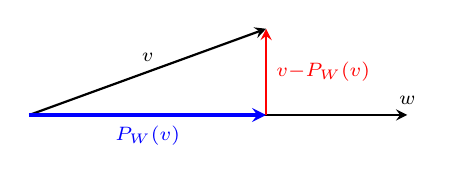
\begin{tikzpicture}[>=stealth,scale=0.8]
                % 1) Main horizontal vector w (length = 6)
                \draw[->, thick] (0,0) -- (6,0)
                     node[pos=1, above] {$\scriptstyle w$};
                % 2) Vector v: 20° angle, length = 4, black
                \draw[->, thick, black] (0,0) -- (20:4)
                     node[midway, above] {$\scriptstyle v$};
                % 3) Projection of v onto w, in blue (a bit thicker)
                %    Projected length = 4*cos(20°), purely along x-axis
                \draw[->, very thick, blue] (0,0) -- ({4*cos(20)}, 0)
                     node[midway, below] {$\scriptstyle P_W(v)$};
                % 4) Vector from the tip of P_W(v) to the tip of v (v - P_W(v)), in red
                \draw[->, thick, red] ({4*cos(20)}, 0) -- (20:4)
                     node[midway, right] {$\scriptstyle v - P_W(v)$};
            \end{tikzpicture}
        \end{center}
    \end{definition}

    \begin{proposition}***
        Let $V$ be an inner product space and $w \in V$ a nonzero vector. Then $P_w(v) \bot v - P_w(v)$.
    \end{proposition}
        \begin{proof}
            
        \end{proof}

    \begin{corollary}***
        Let $V$ be an inner product space and $w \in W$ a nonzero vector. Then $\lnorm v \rnorm_2^2 = \lnorm P_w(v) \rnorm_2^2 + \lnorm v - P_w(v) \rnorm_2^2$.
    \end{corollary}
        \begin{proof}
            
        \end{proof}

    \begin{lemma}[Cauchy-Schwartz Inequality]\label{lemma:c-s-ineq}
        Let $V$ be an inner product space and $v,w \in V$. Then $|\langle v,w \rangle| \leq \lnorm v \rnorm_2 \lnorm w \rnorm_2$.
    \end{lemma}
        \begin{proof}
            The previous corollary gives $\lnorm v \rnorm_2 \geq \lnorm P_w(v) \rnorm_2$. We have that:
                \begin{equation*}
                \begin{split}
                    \lnorm v \rnorm_2 
                    & \geq \lnorm \frac{\langle v,w \rangle}{\langle w,w \rangle}w \rnorm_2 \\
                    & = \frac{|\langle v,w \rangle|}{\lnorm w \rnorm_2^2}\lnorm w \rnorm_2 \\
                    & = \frac{\langle v,w \rangle}{\lnorm w \rnorm_2}.
                \end{split}
                \end{equation*}
            Multiplying both sides by $\lnorm w \rnorm_2$ gives the desired result.
        \end{proof}

    \begin{theorem}
        Let $V$ be an inner product space. Then $(V,\lnorm \cdot \rnorm_2)$ is a normed space.
    \end{theorem}
        \begin{proof}
            Let $v,w \in V$ and $\alpha \in F$. We have that:
                \begin{equation*}
                \begin{split}
                    \lnorm \alpha v \rnorm_2 
                    & = \langle \alpha v , \alpha v \rangle^\frac{1}{2} \\
                    & = \left( \alpha \overline{\alpha}\langle v,v \rangle \right)^\frac{1}{2} \\
                    & = \left( |\alpha|^2 \langle v,v \rangle\right)^\frac{1}{2}\\
                    & = |\alpha|\lnorm v \rnorm_2.
                \end{split}
                \end{equation*}
            Thus $\lnorm \cdot \rnorm_2$ satisfies homogeneity. It follows from the \nameref{lemma:c-s-ineq} that:
                \begin{equation*}
                \begin{split}
                    \lnorm v+w \rnorm_2^2
                    & = \langle v+w,v+w \rangle \\
                    & = \langle v,v \rangle + \langle v,w \rangle + \langle w,v \rangle + \langle w,w \rangle \\
                    & = \lnorm v \rnorm_2^2 + \langle v,w \rangle + \overline{\langle v,w \rangle} + \lnorm w \rnorm_2^2 \\
                    & = \lnorm v \rnorm_2^2 + 2\Re \left( \langle v,w \rangle \right) + \lnorm w \rnorm_2^2 \\
                    & \leq \lnorm v \rnorm_2^2 + 2|\langle v,w \rangle| + \lnorm w \rnorm_2^2 \\
                    & \leq \lnorm v \rnorm_2^2 + 2 \lnorm v \rnorm_2 \lnorm w \rnorm_2 + \lnorm w \rnorm_2^2 \\
                    & = \left( \lnorm v \rnorm_2 + \lnorm w \rnorm_2 \right)^2,
                \end{split}
                \end{equation*}
            where we used the fact that $2\Re (\langle v,w \rangle) = 2|\langle v,w \rangle|$. Squaring both sides proves that $\lnorm \cdot \rnorm_2$ satisfies the triangle inequality. It remains to show positive-definiteness. Suppose $\lnorm v \rnorm_2 = 0$. Then $\langle v,v \rangle = 0$, but since the inner-product is by definition positive-definite, we get that $v = 0_V$.
        \end{proof}

        \begin{center}
            \begin{tikzpicture}
                \draw[thick] (0.3,0) -- (2.3,0);
                \node at (2.39, 0) {$/\,$};
                \node at (2.56, 0) {$/\,$};
                \draw[thick] (2.6,0) -- (4.6,0);
            \end{tikzpicture}
        \end{center}

    \begin{example}
        \phantom{a}
        \begin{enumerate}[label = (\arabic*),itemsep=1pt,topsep=3pt]
            \item $\ell_2^n = F^n$ is an inner product space where $\langle (x_1,...,x_n),(y_1,...,y_n) \rangle := \sum_{j = 1}^n x_j \overline{y_j}$.
            \item $\ell_2$ is an inner product space where $\langle (a_k)_k,(b_k)_k \rangle := \sum_{k = 1}^\infty a_k \overline{b_k}$. Note that:
                \begin{equation*}
                \begin{split}
                    \sum_{k = 1}^n \left|a_k \overline{b_k}\right| 
                    & = \sum_{k = 1}^n |a_k||b_k| \\
                    & \leq \left( \sum_{k = 1}^n |a_k|^2 \right)^\frac{1}{2} \left( \sum_{k = 1}^n |b_k|^2 \right)^\frac{1}{2} \\
                    & \leq \left( \sum_{k = 1}^\infty |a_k|^2 \right)^\frac{1}{2} \left( \sum_{k = 1}^\infty |b_k|^2 \right)^\frac{1}{2} \\
                    & = \lnorm (a_k)_k \rnorm_2 \lnorm (b_k)_k \rnorm_2 \\
                    & < \infty \quad\quad\quad \text{\tiny (Because $(a_k)_k,(b_k)_k \in \ell_2)$.}
                \end{split}
                \end{equation*}
            Since $\sum_{k = 1}^n |a_k \overline{b_k}|$ is increasing and bounded above, the Monotone Convergence Theorem says $\sum_{k = 1}^\infty|a_k \overline{b_k}|$ exists and is finite. Whence $\langle (a_k)_k,(b_k)_k \rangle$ converges.

            \item Recall that $\Tr:M_n(\bfC) \rightarrow \bfC$ is defined by $\Tr(a_{ij}) = \sum_{i  =1}^n a_{ii}$.
            Then $M_n(\bfC)$ is an inner product space where $\langle a_{ij},b_{ij} \rangle := \Tr(b_{ij}^\ast a_{ij})$.

            \item $C([0,1])$ is an inner product space where $\langle f,g \rangle := \int_0^1 f(x) \overline{g(x)}dx$.
        \end{enumerate}
    \end{example}

    

\section{Normed Algebras}
    \begin{definition}
        A \textit{normed algebra} is an algebra $A$ equipped with a norm $\lnorm \cdot \rnorm_A$ such that $\lnorm ab \rnorm_A \leq \lnorm a \rnorm_A \lnorm b \rnorm_A$. If $A$ is unital, we require $\lnorm 1 \rnorm_A = 1$.
    \end{definition}

    \begin{example}
        \phantom{a}
        \begin{enumerate}[label = (\arabic*),itemsep=1pt,topsep=3pt]
            \item $\ell_\infty(\Omega)$ equipped with $\lnorm \cdot \rnorm_u$ is a normed algebra.
            \item $C_c(\bfR)$, $C_0(\bfR)$, and $C([0,1])$ are all normed algebras when equipped with $\lnorm \cdot \rnorm_u$.
            \item $M_n(F)$ equipped with $\lnorm \cdot \rnorm_\text{op}$ is a normed algebra.
            \item If $V$ is a normed space, then $B(V,V)$ with $\lnorm \cdot \rnorm_\text{op}$ is a normed algebra: for $T,S \in B(V,V)$ and $v \in B_V$, we have that
                \begin{equation*}
                \begin{split}
                    \lnorm (T \circ S)(v) \rnorm
                    & \leq \lnorm T \rnorm_\text{op}\lnorm S(v) \rnorm \\
                    & \leq \lnorm T \rnorm_\text{op}\lnorm S \rnorm_\text{op}.
                \end{split}
                \end{equation*}
            Taking the supremum over all $v \in B_V$ gives $\lnorm T \circ S \rnorm_\text{op} \leq \lnorm T \rnorm_\text{op}\lnorm S \rnorm_\text{op}$.

            \item Let $S$ be a group. Equip the algebra $\bfF(S)$ with $\lnorm \cdot \rnorm_1$. We get a normed algebra.
        \end{enumerate}
    \end{example}

    \begin{exercise}
        For $a,b \in \ell_1(\bfZ)$, define $a\ast b :\bfZ \rightarrow F$ by $(a \ast b)(n) = \sum_{k \in \bfZ}a(n-k)b(k)$. Show that $\ell_1(\bfZ)$ with this multiplication is a normed algbera.
    \end{exercise}
    

    




    
    
